
\subsection{Data Preprocessing}

The data pre processing steps used in this paper including the following steps:

\begin{itemize}
    \item Replace the abbreviations with their normal form.
    \item Remove all the stop words.
    \item Lemmatize the words with it's normal form.
\end{itemize}

We will use functions provided by the NLTK library to remove the stop words and lemmatize the words.
Meanwhile, we also use the regular expressions library to replace the abbreviations with their normal form 
to make the data more clean and easy to process.

After the data preprocessing, the data will be tokenized and converted into a format that can be used by the model.

Then the processed data will be split into training(80\%) and testing data(20\%).

\subsection{Email spam text classification process}

The Email spam text classification process is shown in figure 2 below. The process includes the following steps:
\begin{itemize}
    \item Preprocessing the data 
    \item Tokenization
    \item Model building and training
    \item Spam mail classification

\end{itemize}

To check the performance of the models, the models will also be evaluated using the test data mentioned above.

\begin{figure*}[t]
    \centering
    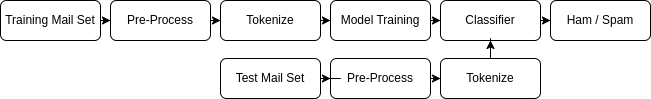
\includegraphics[width=0.8\linewidth]{figure/mail_classification_process.png} \hfill
    \caption{Mail classification process}
\end{figure*}

\subsection{BERT model}

The BERT model used here is a pre-trained model sentence-transformers/bert-base-nli-mean-tokens\cite{reimers-2019-sentence-bert}
which can be downloaded from the huggingface model hub. It contains 2 linear layers with 256 hidden units,
dropout rate set to 0.2,and use RELU function as activation function. Loss function used in BERT model
is Binary Cross Entropy Loss, and optimizer used is Adam optimizer with default learning rate.

\subsection{GPT model}
GPT model, on the other hand, use the pre-trained model gpt2 provided OpenAI\cite{radford2019language}, and it share the same 
SpamClassifier class with the BERT model. However, GPT model are send to GPU instead of CPU, and required
input data are modified to fit the GPT model accordingly. Loss function used in GPT model
is Cross Entropy Loss instead of Binary Cross Entropy Loss, and optimizer used is Adam optimizer with default learning rate.

GPT model contains 2 linear layers with 256 hidden units,
dropout rate set to 0.2, and use RELU function as activation function.

\subsection{Evaluation}

This article uses following four values as evaluation indicators.
1.Accuracy.
2.Precision.
3.Recall.
4.F1-score.
Accuracy represents the spam detection rate, which is the accuracy of 
the model's classification results,
Precision represents the accuracy of the classifier classification,
recall represents the spam detection rate 
and F1 value is a combination of the precision and recall of the classifier, which is the harmonic average of the two, and it is a value between 0 and 1.




